% this file is called up by thesis.tex
% content in this file will be fed into the main document

%: ----------------------- name of chapter  -------------------------
\chapter{The ONE simulator}\label{simulatore} % top level followed by section, subsection


%: ----------------------- paths to graphics ------------------------

% change according to folder and file names
\graphicspath{{5-simulatore/img/}}


%: ----------------------- contents from here ------------------------
The simulation environment chosen for our simulations is The ONE (Opportunistic Network Environment) version 1.4.1\footnote{The ONE simulator \href{http://www.netlab.tkk.fi/tutkimus/dtn/theone/}{http://www.netlab.tkk.fi/tutkimus/dtn/theone/}}, described in \cite{articoloONE}. This simulation environment written in Java is completely configurable and is able to simulate completely the behaviour of nodes in the simulations, including movement, connections and to give a visual feedback about all these factors using its GUI. A more interesting feature, for our purposes, is the capability of emulate message routing using different routing protocols.
\\
 
To emulate nodes movement, the ONE can take in input traces from real-world measurements, from external mobility generators or it can generate movement patterns using synthetic mobility model generators. Differences between several available mobility are explained in Section \ref{movimento}. One characteristic of the ONE architecture is high modularity. Each movement models and for each routing protocol is implemented in an independent module, which is dynamically loaded depending on the simulation settings. This allows a relatively easy implementation of new mobility models and routing protocols in the simulator.
\\

The simulator allows to save data of interest from completed simulations into report files. There reports are created using modules dynamically loaded as it would happen with movement and routing modules.
\\

\section{Configuration}
\label{configurazioneONE}
A single simulation is set, before running, using configuration files which describe the simulated environment, from the simulation length to number of nodes emulating people in the simulated environment. Configuration files are text-based files that include parameters about the simulation, user interface, event generation, and reporting modules. All these parameters are loaded before the beginning of simulations and are used to adjust details about the behaviour of loaded modules.
\\

%Many of the simulation parameters are configurable separately for each node group but groups can also share a set of parameters and only alter the parameters that are specific for the group. The configuration system also allows defining of an array of values for each parameter hence enabling easy sensitivity analysis: in batch runs, a different value is chosen for each run so that large amounts of permutations are explored.

Inside configuration files, parameters are saved as key-value pairs and syntax for most of the
variables is:

\begin{center}
\textit{Namespace.key = value}
\end{center}

Namespace defines the part of the simulation environment where the setting has effect on. Many, but not all, namespaces are equal to the class name where they are read. This convention is especially followed by movement models, report modules and routing modules, so also created new modules should follow it.
\\

To make human-readability and configuration easier, numerical values can use suffixes kilo (k), mega (M) o giga (G), with \textquotedblleft .\textquotedblright \ as decimal separator. Boolean parameters accept \textquotedblleft true\textquotedblright \
 or \textquotedblleft 1\textquotedblright , \textquotedblleft false\textquotedblright \ or \textquotedblleft 0 \textquotedblright .
\\
 
Setting files can include comments with \textquotedblleft
\#\textquotedblright \ character. Rest of the line is skipped when the settings are read.
\\

Every simulation can be set using several configuration files, to divide parameters into different categories, e.g. a file can include scenario parameters, like maps, streets and districts, another file can include parameters used to configure nodes, another file can include reports configuration and so on. First configuration file read, if exists, is always \textquotedblleft default\_settings.txt\textquotedblright. Other configuration files given as parameter can define more settings or override some (or even all) settings in the previous files. The idea is that you can define in the earlier files all the settings that are common for all the simulations and run different simulations changing parameters only in latests configuration files.
\\

The basic agents in the simulator are called nodes. A node models a mobile endpoint capable of acting as a store-carry-forward router (e.g., a pedestrian, car or tram with the required hardware). Nodes in the simulation world are divided into groups, each one configured with different capabilities. Inside a group, every node has the same characteristics, i.e. radio interface, persistent storage, movement, energy consumption and message routing protocol. It is possible to configure some of these capabilities as common for all groups, avoiding to set them individually for each group. Changing some configuration value between a group and another, allows to get heterogeneity between the behaviour of nodes in simulated scenario.
\\

In configuration files is also possible to provide an array of settings for every parameter. This allows to run large amounts of different simulations using only one single configuration file. Every simulation will be different from the previous and this is very useful to gather reports about different aspects in a common scenario.
\\ Syntax for these configuration parameters is

\begin{center}
\textit{Namespace.key = [run1\_value; run2\_value; run3\_value; etc]}
\end{center}

Some parameters, finally, accept a file path as value and this can be either an absolute or relative path. These parameters are used for maps, nodes paths or events to be loaded by event generators modules.

\section{Simulation outputs}
The main way to follow the progress of simulations is the GUI present in the ONE. In main window, shown in Fig.\ref{Schermata-ONE}, is possible to observe movements of nodes acting in the simulation and view details about one of them by selecting it from the list of active nodes. For every node is possible to get informations about active connections, messages carried and other details. In the main window is also present a log panel updated with a textual description of events generated in the current simulation. These events can be filtered allowing to see only logs related to one kind of events e.g. new connections, creation of messages or massage exchanges.
\\
\begin{figure}[htpb]
  \begin{center}
    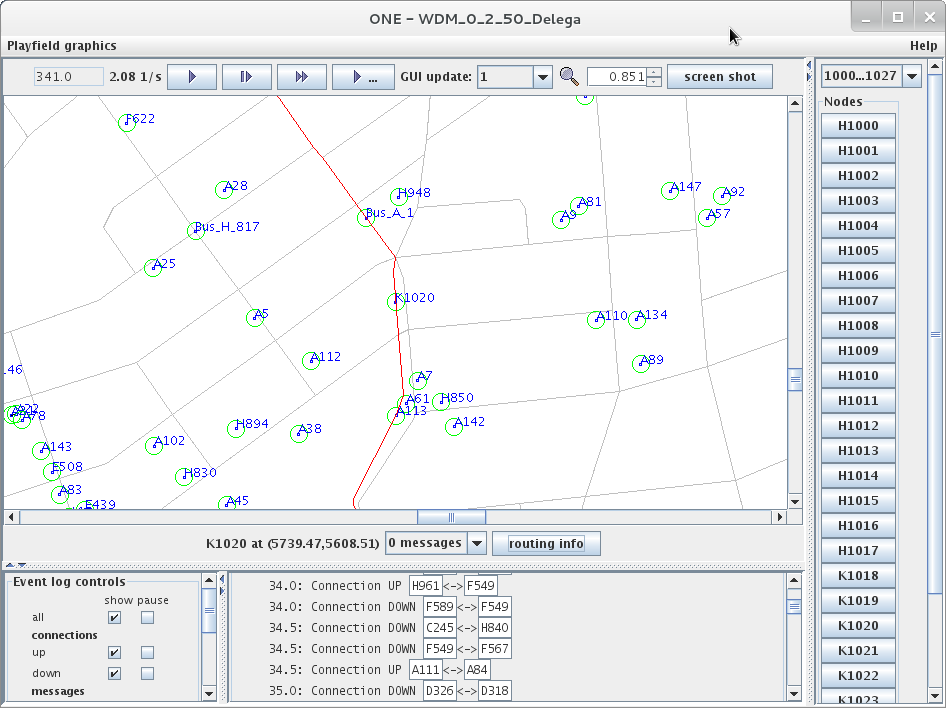
\includegraphics[scale=0.4]{5-simulatore/img/Schermata-ONE.png}
    \caption[Main window]{Main Window of the ONE}    
    \label{Schermata-ONE}
  \end{center}
\end{figure}
%\figuremacro{Schermata-ONE}{Schermata Principale}{La schermata principale del simulatore ONE}{}

Selecting a node is also possible to follow its movements inside the simulated world map, with the path to its next destination highlighted in the graphical visualization of the map. A pop-up window, shown in Fig. \ref{Routing-Info}, can be invoked to get advanced informations about the state of that node.
\\

\begin{figure}[htpb]
  \begin{center}
    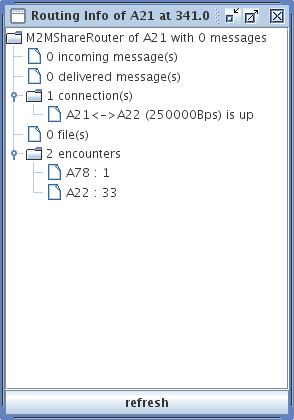
\includegraphics[scale=0.6]{5-simulatore/img/Routing-Info.png}
    \caption[Routing Info]{Example of detail window related to a node state}    
    \label{Routing-Info}
  \end{center}
\end{figure}
%\figuremacro{Routing-Info}{Routing Info}{Un esempio di finestra in cui sono presenti i dettagli relativi allo stato di un nodo}{}

The map representation is configurable and the user can adjust the zoom level, simulation speed and it's possible to add an image as background, e.g. using a road map or a satellite photo of the interested area.
\\

The other way to follow the progress of simulations is to read generated reports, at the end of every simulation. Each report is generated by its related module. These modules, like movement and routing modules, are dynamically loaded at the beginning of the simulation according to what set in configuration files. To use report files is particularly useful when doing simulations in batch, without using the GUI and analysing resulting reports when all the set of simulations is complete. In batch mode is useful the possibility of define arrays of values for parameters in configuration files. These allow to set differences in configuration between the different runs of the batch. When the batch is executed, the ONE would run all the simulations, reading for each of them the correct configuration parameters, and saving the generated reports into different files for each simulation run.
\\

Several report modules can be active during one single simulation. Output of these modules are report files, which typically are text-based files in which are saved statistical and log data gathered during the simulation. These data can be further analysed when the simulation has ended. In the ONE version 1.4.1, the simulator has some ready-to-use report modules which allow to create reports related to:

\begin{description}
\item[messages,] e.g. number of created messages, delivery times, expired messages, etc..
\item[contacts,] which can show contact and inter-contact time between the nodes, or the number of contacts during the simulation
\item[connections,] which can show changes in connections status
\end{description}

Report modules are handled by the simulator like other modules and this allows to easily implement and add new report modules to the simulator, to gather needed data from simulations.


\section{Simulation execution}
\label{esecuzioneONE}
It can be interesting to explain in detail how a single simulation is run by the simulator. Let's see what steps are performed for each run.
\\

The first step done is configuration loading. The simulator read from configuration files values assigned to simulation parameters. Configuration files path are passed as arguments to the ONE launch command. When a configuration file is read, values included are used to initialize or overwrite the value of some variables in simulation environment. If some parameters value is not set in configuration files, default values are used and an exception is thrown if a default value was not present for that parameter.
\\

When the simulation is configured, the creation of the simulated scenario begins. In the scenario are included all active entities in the simulation, i.e. nodes, report generators or event generators, and passive entities, i.e. maps which composes the simulated world. In this phase all nodes are created and initialized according to the loaded configuration. Every node includes a router implementing one routing protocol, uses one movement model and has some \textit{listener} associated used to catch events and generate reports.
\\

When all entities operating in the simulation are created an configured, the main phase of the simulation begins. This consists in an iterative update of the status of simulated world, obtained by calling a method \textit{update()}, and increasing simulation clock value. This clock measure how much time is passed from the beginning of the simulation and incremental step value is configurable in configuration files, using the parameter \textit{Scenario.updateInterval}. This accept a double value and it indicates how many seconds wait between an update of the world and the next one. This value have a big influence over results of the simulation. This because a simulation with a small \textit{updateInterval} would be more accurate than one with a big value of update, having a more frequent update of the status of simulate world, but it also need more computational time to complete the simulation.
\\

The first action executed in simulated world \textit{update()} is to move nodes inside the simulation map. This is done according to every node's movement model and to \textit{Scenario.updateInterval} value. E.g. a node simulating a car driver will move farther than a node simulating a pedestrian, considering the same \textit{updateInterval} time value. As we saw in Section \ref{movimento}, related to movement models, these models can be very complex and can simulate several different movement behaviours, according to configuration values used.
\\

When it has been moved, for every node are updated connections and simulated router status. For every network interface is checked if the movement just occurred has changed its status, i.e. some connection has been closed because the two end points are now out of range or some new connection has been established. When the status of a connection changes, related \textit{listeners} are informed, report modules are informed too, if enabled, and GUI is updated showing changes in connection status, as shown in Figure \ref{connessioni}.
\\
\figuremacro{connessioni}{Connections}{An example of graphical representation of connection between nodes. In the left side is shown an active connection, while in the right side nodes are no more in communication range, represented by the circle around them.}{}

Last action performed during simulated world \textit{update()} is to update router status for every node. This part is strongly dependent on routing protocol simulated and, by overriding router module \textit{update()} method, is the way to implement a new routing protocol in the ONE.

\section{Randomness}
\label{randomness}
One basic characteristic of a simulation done with a network simulator like the ONE is repeatability, i.e. running several simulations with the same configuration, results of these simulations will be the same, as will be the same the behaviour of acting nodes in the simulations. This is fundamental to verify correctness of data and results of completed simulations, or to repeat the simulation changing only few parameters over the total configuration, leaving constant the simulated world description.
\\

To achieve a statistical correctness in analysis, we need to repeat a simulation several times, to get results independent from initial position and movement of nodes. Doing average analysis over simulations results, allows to study statistical trend of analysed variables, without focusing to best or worst cases that can happen during several simulations. 
\\

To achieve that result, each movement models modules uses a \textit{random number generator}. This generator is initialized with a long type seed, read from configuration files as value for the parameter \textit{MovementModel.rngSeed}. The seed is the initial value of the internal state of the pseudorandom number generator which is maintained by method \textit{next}. In details, if two instances of random generator are created with the same seed, and the same sequence of method calls is made for each, they will generate and return identical sequences of numbers. This means that if the seed and all the movement model related settings are kept the same, all nodes should move the same way in different simulations (same destinations, speed and wait time values are used).
\\

This is the strategy we used to get an high number of related simulations, from which we got results later analysed: we keep constant all simulation settings, specified by one configuration file and we change, for every run, \textit{MovementModel.rngSeed} value. Doing so we got data to analyse, from reports, independent from initial position and movements of nodes. 


\section{The map}
\label{mappaONE}
The map defines the space and routes in which the nodes can move inside the simulated world. The design of the map is an important part of the mobility model because it includes all the information of the locations of the houses, offices and meeting spots, as well as bus routes with bus stops. Since all the movement of the nodes is determined by activities with specific locations, the placement of these locations define how nodes are moving on a larger scale. Locations can be node group specific, i.e. some offices are used only by nodes in one group, nodes in different groups live in different houses locations, etc.. This makes it possible to create small districts within the map. For our simulations we used one map included in the ONE. It is the map of Helsinki city centre and surrounding districts, with size of about 8000 x 7000 m$^{2}$. In Fig. \ref{imgMappaABCD} is shown the map and it is possible to see the four main district in which the map is divided. 

\begin{figure}[htpb]
  \begin{center}
    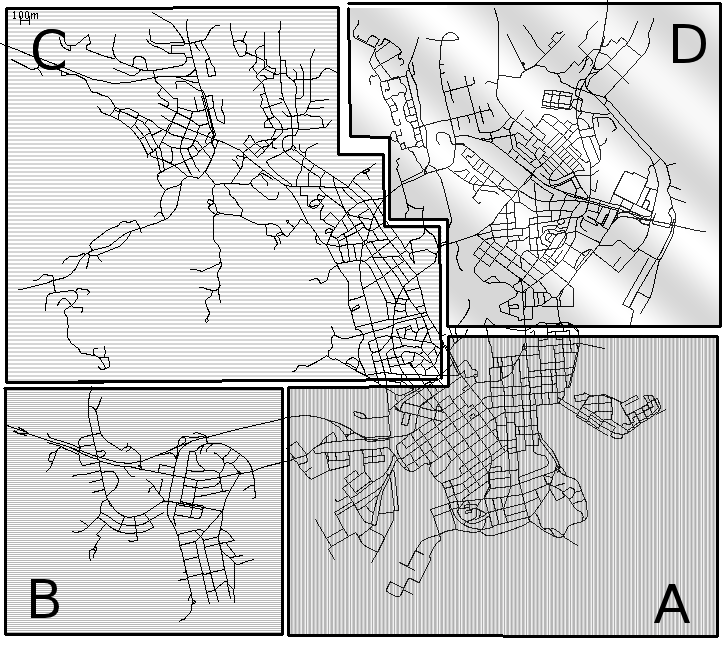
\includegraphics[scale=0.5]{figure/mappa_ABCD.png}
    \caption[Helsinky map]{The map of the Helsinki centre area used in our simulations}    
    \label{imgMappaABCD}
  \end{center}
\end{figure}


In this implementation, every node group belongs to a district i.e. all nodes in one group will have their home location, office and meeting spot inside the related district. This is useful to limit node movement to small areas. Doing this we increased locality and it is not possible that nodes belonging to different groups (and so different districts) can meet each others. To decrease locality it is possible to spread houses, offices and meeting spots on the map, having nodes meeting easily.
\\

It is also possible to combine low and high locality: in Helsinki map used for our simulations there are four main districts, with different sizes, overlapped by other districts. This allows to have high locality but also some movement between districts, which corresponds to nodes coming to some district to work or meet friends, while others are leaving their district for similar reasons. Nodes moving between districts, not located next to each other, will have to pass through other districts. 
\\

\begin{table}[h]
\begin{center}
\begin{tabular}{|l|c|c|c|}
\hline
\textbf{District} & \textbf{Nodes} & \textbf{Offices} & \textbf{Meeting spots}\\
\hline
\hline
\bfseries A & 150 & 30 & 4 \\
\hline
\bfseries B & 50 & 10 & 1 \\
\hline
\bfseries C & 100 & 20 & 2 \\
\hline
\bfseries D & 100 & 20 & 2 \\
\hline
\bfseries E (A + B) & 100 & 20 & 2 \\
\hline
\bfseries F (A + C) & 150 & 30 & 4 \\
\hline
\bfseries G (A + D) & 150 & 30 & 4 \\
\hline
\bfseries H (Whole map) & 200 & 40 & 5 \\
\hline
\end{tabular}
\end{center}
\caption[Helsinky map districts]{Table showing assignment of nodes, offices and meeting spots between districts in Helsinky map}    
\label{tabellaDistrettiMappa}
\end{table}

In Table \ref{tabellaDistrettiMappa} is shown distribution of nodes, offices and meeting spots in the districts of the map. Every district has its own bus route with 2 busses running on it. The only exception is district H which has 4 busses running on its route. This is done because the district covers the entire map and with only 2 busses the waiting times would be too much long.

%
%\section{Limitations}
%\label{limitazioniONE}
%non più in basso del livello di routing
%simulazione temporale discreta
%mancanza di simulazione di un file system




% ---------------------------------------------------------------------------
%: ----------------------- end of thesis sub-document ------------------------
% ---------------------------------------------------------------------------

